\newpage

\section{Программная реализация}

В данном разделе представлено описание выбранных инструментов разработки для решения поставленной задачи. 
Описана программная реализация модуля интерпретации предметно-ориентированного языка.
Рассмотрены детали реализации его основных структурных частей.
Также выполнено тестирование основных функций программы.

\subsection{Выбор инструментов разработки}

В качестве языка программирования для разработки был выбран Go.

Go (Golang) -- это компилируемый многопоточный язык программирования с открытым исходным кодом, разработанный компанией Google \refref{ref:golang}.

Выбор данного языка обусловлен совместимостью между разрабатываемым модулем и основной системой,
так как для реализации серверной части конструктора Telegram ботов так же был выбран язык Go.
Использование одного языка для всей системы гарантирует,
что модули будут легко интегрироваться друг с другом без необходимости создания сложных интерфейсов или адаптеров.

Язык Go имеет и другие положительные характеристики:
\begin{itemize}
    \item высокая производительность -- Go компилируется в машинный код, что обеспечивает его высокую скорость исполнения;
    \item безопасность типов -- строгая статическая типизация предотвращает множество ошибок на этапе компиляции;
    \item встроенная поддержка параллелизма -- в Go реализованы горутины и каналы -- встроенные механизмы для эффективной работы с параллельными задачами;
    \item расширяемость -- язык имеет встроенную систему управления модулями и широкую экосистему общедоступных библиотек.
\end{itemize}

Выбор языка программирования Go для реализации модуля интерпретации предметно-ориентированного языка конструктора Telegram ботов обоснован тем,
что он позволяет поддерживать единообразие кода, использовать его технические преимущества и соответствовать основным требованиям проекта.

\subsection{Реализация лексического анализатора}

Лексический анализатор состоит из следующих основных компонентов:
\begin{itemize}
    \item токены -- определение структуры и типов токенов, представляющих основные элементы языка;
    \item конечный автомат -- принимает на вход поток символов и определяет токены переходя между состояниями в соответствии с правилами языка.
\end{itemize}

Токен представляет собой структуру, содержащую информацию о типе токена и его значение, представленное в виде строки.
Код структуры, представляющей токен приведен на рисунке~\ref{f:code_tokenStruct}.

\begin{figure}[ht]
	\centering
	\vspace{\toppaddingoffigure}
	\begin{lstlisting}[
        language=Go
    ]
type TokenType = string
type Token struct {
    Type    TokenType
    Literal string
}        
\end{lstlisting}
	\caption{Структура, представляющая токен}
	\label{f:code_tokenStruct}
\end{figure}

Список возможных токенов рассмотрен ранее, см. таблицу~\ref{t:tokens}.

Программную реализацию токенов можно выполнить с помощью списка константных значений.
Фрагмент кода реализации токенов представлен на рисунке~\ref{f:code_tokensFragemnt}.

\begin{figure}[ht]
	\centering
	\begin{lstlisting}
IDENT  = "IDENT"  // x, t, add
INT    = "INT"    // 123
STRING = "STRING" // "abcde"
ASSIGN = "="
PLUS   = "+"
STAR   = "*"
LT  = "<"
GT  = ">"
LAND = "&&"
LOR  = "||"

// keywords
IF     = "IF"
ELSE   = "ELSE"
TRUE   = "TRUE"    
\end{lstlisting}
	\caption{Фрагмент кода реализации токенов}
	\label{f:code_tokensFragemnt}
\end{figure}

Лексер представляет собой структуру, содержащую информацию о входной строке кода,
текущем считанном символе, позиции курсора и других технических значениях, необходимых для корректной работы анализатора.
Структура представляющая лексер приведена на рисунке~\ref{f:code_lexerStruct}.

\begin{figure}[ht]
	\centering
	\vspace{\toppaddingoffigure}
	\begin{lstlisting}[
        language=Go,
        xleftmargin=.08\textwidth,
        xrightmargin=.08\textwidth
    ]
type Lexer struct {
    input   string
    ch      byte // current char
    pos     int  // current position (on current char)
    readPos int  // position after current char
    nlsemi  bool // if "true" '\n' translate to ';'
    loPos   token.Pos
}    
\end{lstlisting}
	\caption{Структура, представляющая лексер}
	\label{f:code_lexerStruct}
\end{figure}

Основная функция лексического анализатора может быть реализована в формате конечного автомата.
При получении очередного символа из входной строки кода его необходимо сопоставить с одним из токенов.
Стоит заметить, что некоторые токены формируются за счет двух и более символом, например токен <<LAND>> (\&\&), идентификаторы, ключевые слова и т.д. 
В этом случае, необходимо продолжать получение символов из входной строки до тех пор, пока не будет однозначно определен токен.

Основная функция определения токена выполнена в виде конструкции switch-case.
Фрагмент кода представлен на рисунке~\ref{f:code_lexerFragment}.

\clearpage

\begin{figure}[!ht]
	\centering
    \begin{lstlisting}[
        language=Go,
        xleftmargin=.08\textwidth,
        xrightmargin=.08\textwidth
    ]
func (l *Lexer) NextToken() (token.Token, token.Pos) {
    l.skipWhitespace()
    nlsemi := false
    var tok token.Token
    switch l.ch {
    case '\n':
        tok = newToken(token.SEMICOLON, l.ch)
    case '=':
        if l.peekChar() == '=' {
            l.readChar()
            literal := "=="
            tok = token.Token{Type: token.EQ, Literal: literal}
        } else {
            tok = newToken(token.ASSIGN, l.ch)
        }
    case '+':
        tok = newToken(token.PLUS, l.ch)
    case '-':
        tok = newToken(token.MINUS, l.ch)
    case '*':
        tok = newToken(token.STAR, l.ch)
    case '/':
        tok = newToken(token.SLASH, l.ch)
    case '!':
        if l.peekChar() == '=' {
            l.readChar()
            literal := "!="
            tok = token.Token{Type: token.NEQ, Literal: literal}
        } else {
            tok = newToken(token.EXCLAMINATION, l.ch)
        }
    case '%':
		tok = newToken(token.PERCENT, l.ch)
	case '<':
		if l.peekChar() == '=' {
			l.readChar()
			literal := "<="
			tok = token.Token{Type: token.LEQ, Literal: literal}
		} else {
			tok = newToken(token.LT, l.ch)
		}
\end{lstlisting}
	\caption{Фрагмент кода лексера}
	\label{f:code_lexerFragment}
\end{figure}
\subsection{Разработка синтаксического анализатора}

% В данном разделе необходимо выполнить разработку алгоритмов функционирования синтаксического анализатора.

Синтаксический анализ – процесс сопоставления последовательности токенов с формальной грамматикой языка.
Результатом работы синтаксического анализатора является абстрактное синтаксическое дерево (AST),
которое отражает синтаксическую структуру входной последовательности и содержит всю необходимую информацию для дальнейших этапов работы транслятора.

В задачу синтаксического анализа входит поиск и выделение основных синтаксических конструкций текста входной программы,
установление типа и проверка правильности каждой синтаксической конструкции, а так же представление их в виде AST.

Существует два основных метода синтаксического анализа:

\begin{itemize}
    \item нисходящий;
    \item восходящий.
\end{itemize}

В данном проекте реализован нисходящий анализатор, работающий по методу рекурсивного спуска,
известный как парсер Пратта, который впервые описал Вон Пратт в статье «Нисходящий парсер с операторным предшествованием».

Этот метод основан на идее приоритета операторов и обработке различных уровней приоритета в выражениях.
В парсере Пратта каждый оператор имеет свой уровень приоритета.
Операторы с более высоким приоритетом связываются с операндами сильнее, чем операторы с более низким приоритетом.
Значения приоритетов для каждого оператора разрабатываемого предметно-ориентированного языка показаны в таблице~\ref{t:operator_priority}.

\clearpage

\begin{table}[h!]
    \Large
    \caption{Приоритеты операторов}
    \label{t:operator_priority}
    \centering
    \begin{tabularx}{\textwidth}{|c|X|}
        \hline
        Приоритет & Операторы             \\
        \hline
        0         & Минимальный приоритет \\
        \hline
        1         & =                     \\
        \hline
        2         & | |                   \\
        \hline
        3         & \&\&                  \\
        \hline
        4         & == !=                 \\
        \hline
        5         & < > <= >=             \\
        \hline
        6         & + -                   \\
        \hline
        7         & * / \%                \\
        \hline
        8         & -x or !x              \\
        \hline
        9         & (                     \\
        \hline
        10        & [                     \\
        \hline
    \end{tabularx}
    \vspace{\bottompaddingoftable}
\end{table}

Для примера работы приоритета операторов рассмотрим пример построения AST для арифметического выражения: $3 + 1 * 4 * 6 + 8$.
Диаграмма, показывающая рекурсивные вызовы для формирования выражений к приведенному примеру изображена на рисунке~\ref{f:priorities}.

\begin{figure}[ht]
	\centering
	\vspace{\toppaddingoffigure}
	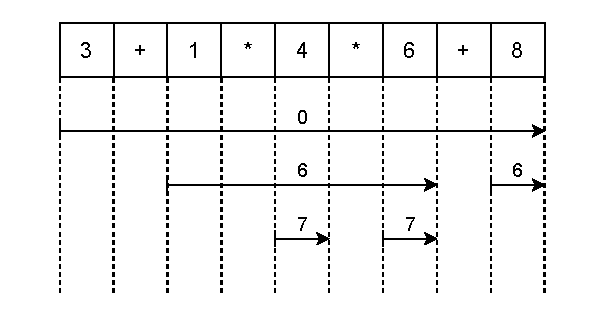
\includegraphics[width=0.7\textwidth]{structures/parser/priorities.pdf}
	\caption{Диаграмма рекурсивных вызовов}
	\label{f:priorities}
\end{figure}

Над стрелками обозначены приоритеты операторов, к которым относится эта стрелка.
В самом начале распознавания выражения значение приоритета равняется 0.
По мере обнаружения оператора, приоритет которого выше текущего алгоритм переходит на следующий уровень рекурсии.
По диаграмме видно, что справа от первого оператора «+» длинная стрелка с приоритетом 6, группирует члены умножения, так как операция умножения имеет больший приоритет, чем сложение.
Эта стрелка заканчивается перед последним «+», так как приоритет оператора, относящегося к этой стрелке не ниже приоритета последнего «+».
Другими словами, экземпляр выражения с более низким приоритетом ожидает результата формирования выражения с более высоким приоритетом.

Абстрактное синтаксическое дерево для данного примера приведено на рисунке~\ref{f:ast_example}.

\begin{figure}[ht]
	\centering
	\vspace{\toppaddingoffigure}
	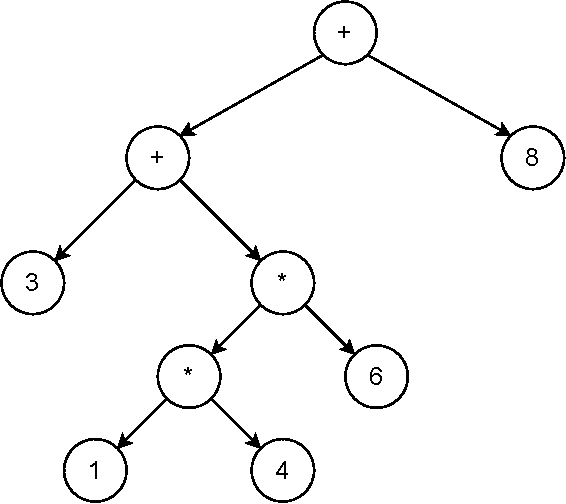
\includegraphics[width=0.7\textwidth]{structures/parser/ast_example.pdf}
	\caption{Абстрактное синтаксическое дерево}
	\label{f:ast_example}
\end{figure}

Некоторые схемы алгоритма построения абстрактного синтаксического дерева представлены на рисунках~\ref{f:parse_program}~-~\ref{f:parse_Expression}.

% В данном разделе была выполнена разработка структурных решений и алгоритмов функционирования синтаксического анализатора.

\clearpage

\begin{figure}[!htp]
	\centering
	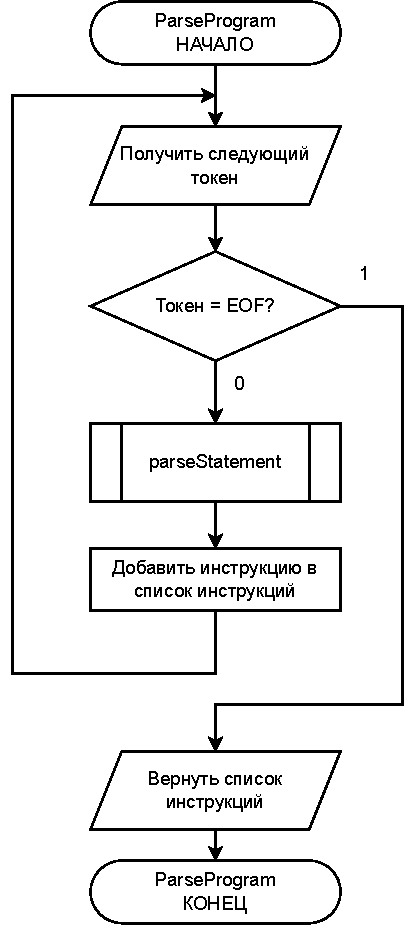
\includegraphics[width=0.5\textwidth]{structures/parser/parse_program.pdf}
	\caption{Схема алгоритма «ParseProgram»}
	\label{f:parse_program}
\end{figure}

\clearpage

\begin{figure}[!htp]
	\centering
	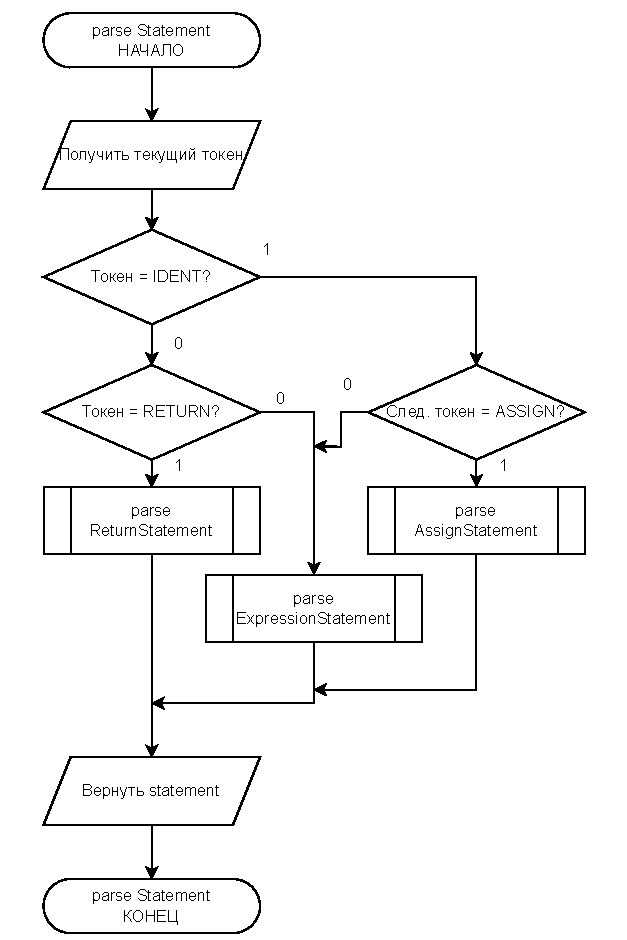
\includegraphics[width=0.7\textwidth]{structures/parser/parse_statement.pdf}
	\caption{Схема алгоритма «parseStatement»}
	\label{f:parse_statement}
\end{figure}

\clearpage

\begin{figure}[!htp]
	\centering
	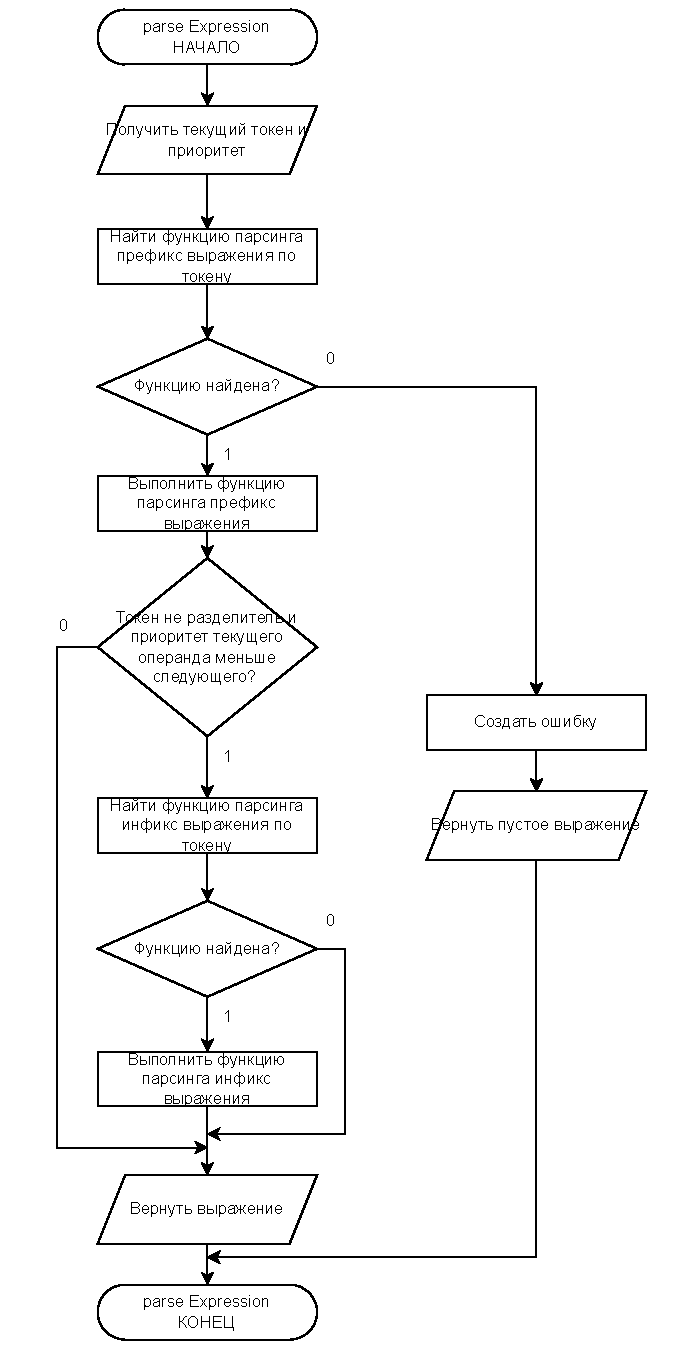
\includegraphics[width=0.60\textwidth]{structures/parser/parse_Expression.pdf}
	\caption{Схема алгоритма «parseExpression»}
	\label{f:parse_Expression}
\end{figure}

\clearpage


\subsection{Разработка семантического анализатора}

% В данном разделе необходимо выполнить разработку алгоритмов функционирования семантического анализатора.

Семантический анализ – это этап работы транслятора, вот время которого выполняется проверка текста исходной программы с точки зрения семантики языка.
В ходе семантического анализа выполняется такие операции, как проверка типов данных, правильность использования переменных, функций, выражений, а также обнаружение смысловых ошибок в коде.

Обобщенная модульная структура серверной части конструктора представлена на рисунке~\ref{f:modules_server_struct}.

Процесс семантического анализа выполняется после построения абстрактного синтаксического дерева синтаксическим анализатором.
Семантический анализ сгруппирован с этапом исполнения выражений.
Таким образом при одном проходе AST алгоритм выполняет проверку узла дерева на семантическую корректность и переход к его исполнению,
если не было обнаружено ошибок при семантическим анализе. В случае обнаружения семантической ошибки возвращается информация о ней,
а процесс интерпретации переход к следующему выражению.

На этапе проектирования семантического анализатора закладываются решения, которые лягут в основу принципов написания кода на разрабатываемом языке.
Например, на этапе построения семантического анализатора, нужно решить, как будет обрабатываться значение в условном выражении, не имеющее тип boolean.
Есть несколько вариантов обработки таких значений.
Один из них - всегда принимать данное значение за «false» и идти в соответствующую ветвь.
В ином случае, при обнаружении значения с типом, отличным от boolean необходимо вернуть ошибку и прекратить выполнение данного выражения.
В этом проекте будет использован второй вариант с возвратом ошибки.

Семантический анализатор принимает на вход элементы абстрактного синтаксического дерева.
После проверки семантической корректности выражения AST, следует его вычисление.
Результаты вычислений выражений, как промежуточные, так и окончательные необходимо каким-то образом представить в памяти.
Это необходимо в первую очередь для получения ранее вычисленных выражений и работы с ними.
В качестве примера можно рассмотреть код, представленный на рисунке~\ref{f:code_example_var}.

\begin{figure}[ht]
	\centering
	\vspace{\toppaddingoffigure}
	\begin{lstlisting}
X = 5;
X + 3
\end{lstlisting}
	\caption{Пример кода использования объявленной переменной}
	\label{f:code_example_var}
\end{figure}

В первой строке присваивается значение 5 переменной «X».
Затем выполняется выражение «X + 3».
Чтобы получить значение данного выражения нужно получить ранее вычисленное значение 5.
Для этого необходимо как-то сохранить его в памяти.

Решение данной задачи состоит в введении внутреннего представления вычисленных значений на время семантического анализа и этапа исполнения.
Примем некоторую объектную систему, состоящую из набора объектов, каждый из которых будет содержать информацию о представляемом им типе данных в предметно-ориентированном языке.

Каждый объект должен содержать информацию о значении представляемого им типа данных предметно-ориентированного языка.
Кроме этого, необходимо реализовать возможность определения того, какой тип данных предметно-ориентированного языка представляет объект, а также функционал получения строкового значения объекта.
Кроме этого, типы данных: целое число, строка и булево значение могут использоваться в виде ключей в хэш-карте.
Для этого необходимо специально для объектов, представляющих эти типы предусмотреть функцию вычисления хэш строки от их значения. 

Объектная система должна представлять все типы данных предметно-ориентированного языка, а именно:
целые числа, строки, булевы значения, массивы, хэш-карты.
Также необходимо ввести дополнительные объекты, представляющие семантические ошибки, значение «null», функции, операцию возврата значения из функции.

Объектная система может быть представлена в виде диаграммы классов.
Диаграмма классов представлена на рисунке~\ref{f:class_diagram}.

\clearpage

\begin{figure}[!htp]
	\centering
    \vspace{\toppaddingoffigure}
	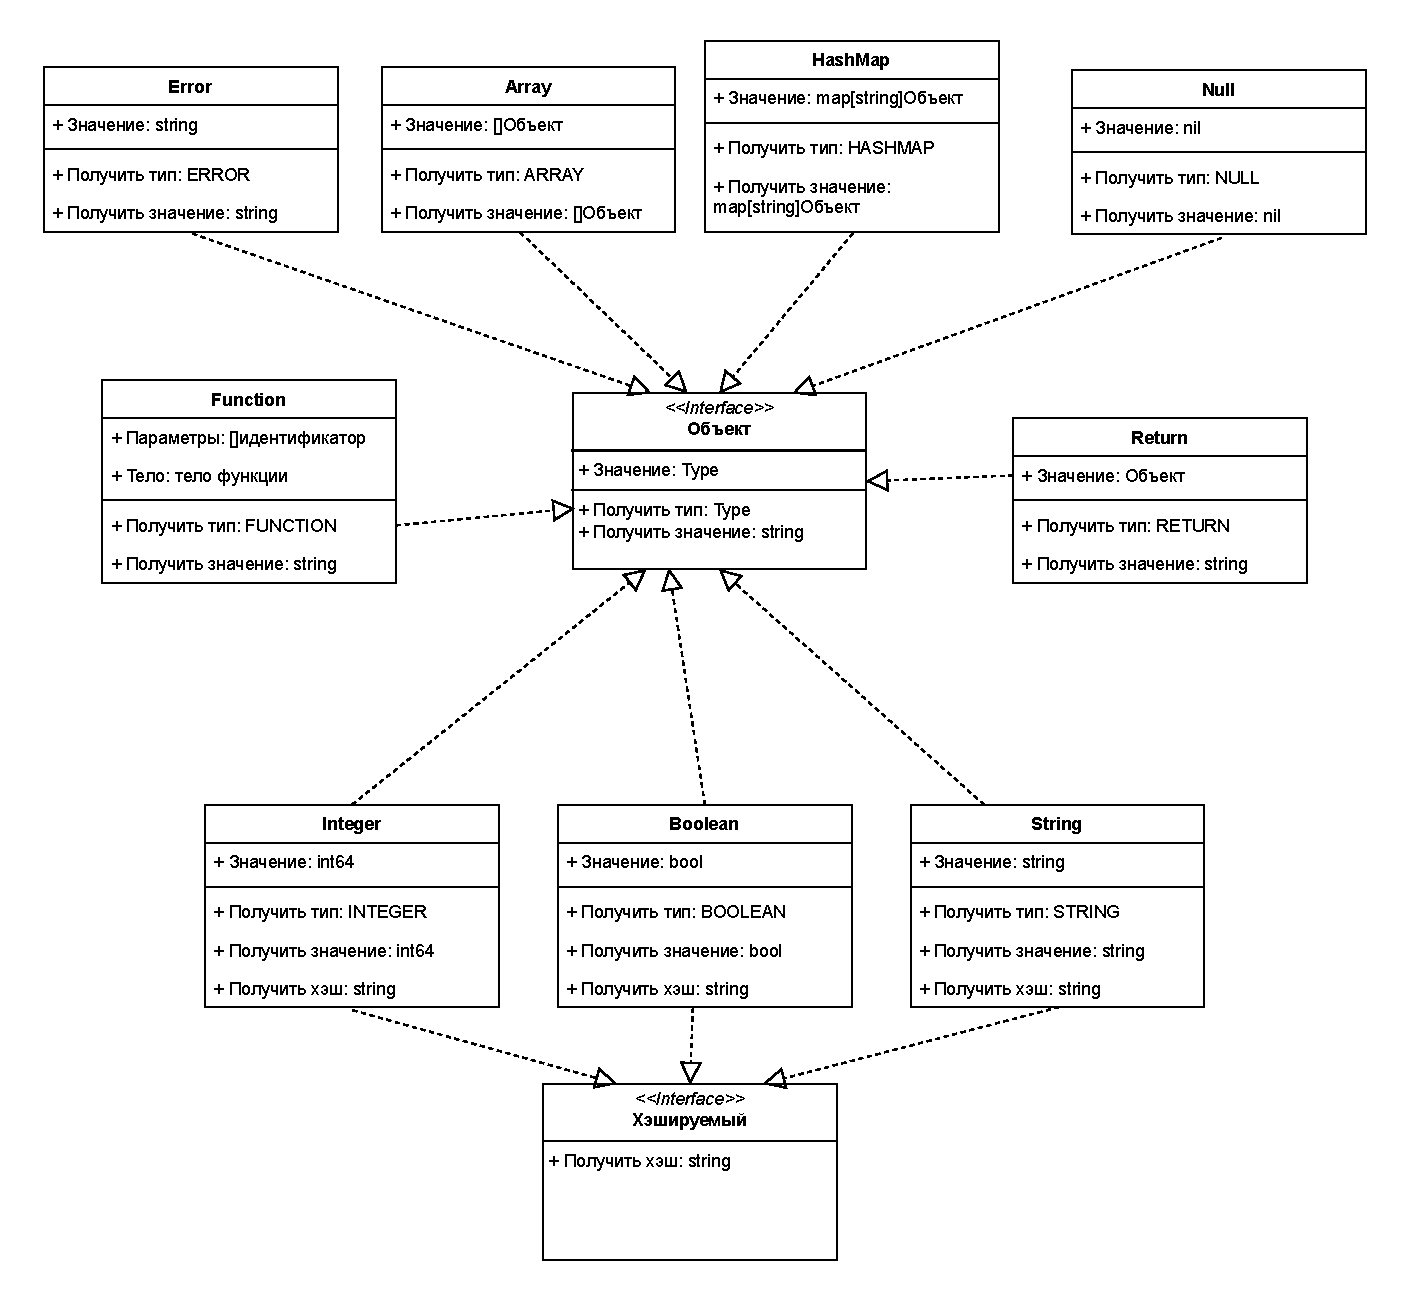
\includegraphics[width=1.0\textwidth]{structures/semantic_analyzer/class_diagram.pdf}
	\caption{Диаграмма классов}
	\label{f:class_diagram}
\end{figure}

В качестве примера работы алгоритма на рисунках~\ref{f:evalProgram}~-~\ref{f:semantic_index_expr} приведены схемы алгоритмов семантического анализа некоторых выражений.

% В данном разделе была выполнена разработка структурных решений и алгоритмов функционирования семантического анализатора.

\begin{figure}[!htp]
	\centering
	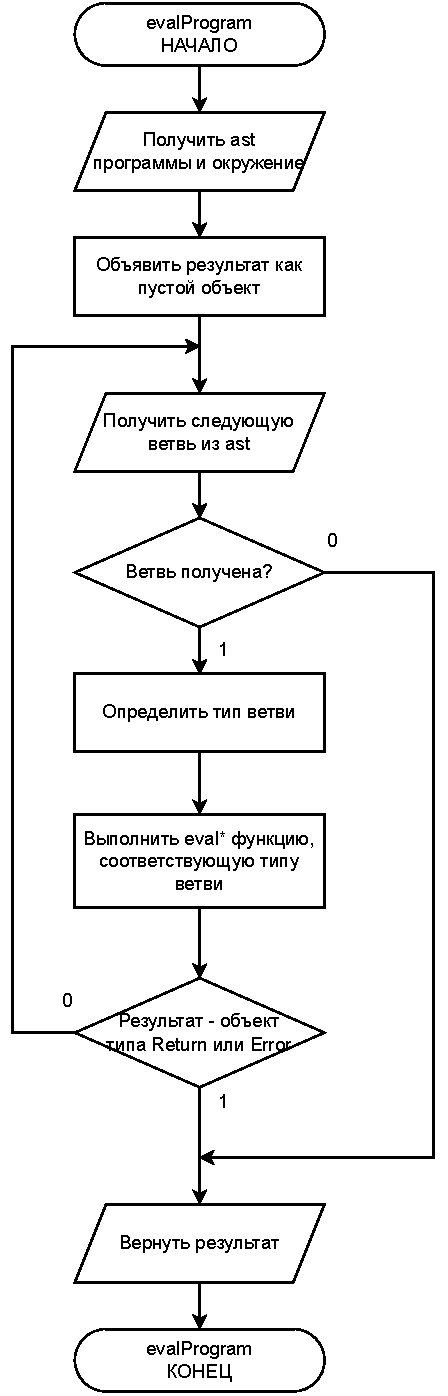
\includegraphics[width=0.4\textwidth]{structures/semantic_analyzer/semantic_Program.pdf}
	\caption{Схема алгоритма «evalProgram»}
	\label{f:evalProgram}
\end{figure}

\clearpage

\begin{figure}[!htp]
	\centering
	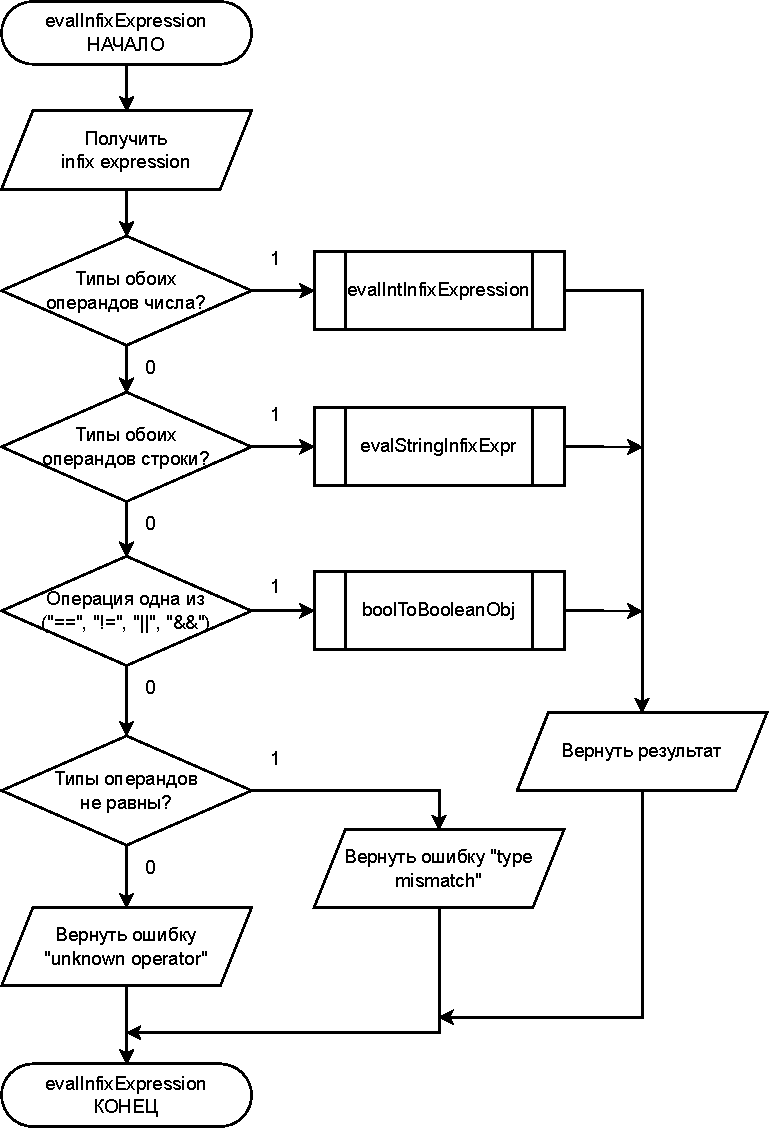
\includegraphics[width=0.9\textwidth]{structures/semantic_analyzer/semantic_infix_expr.pdf}
	\caption{Схема алгоритма «evalInfixExpression»}
	\label{f:semantic_infix_expr}
\end{figure}

\clearpage

\begin{figure}[!htp]
	\centering
	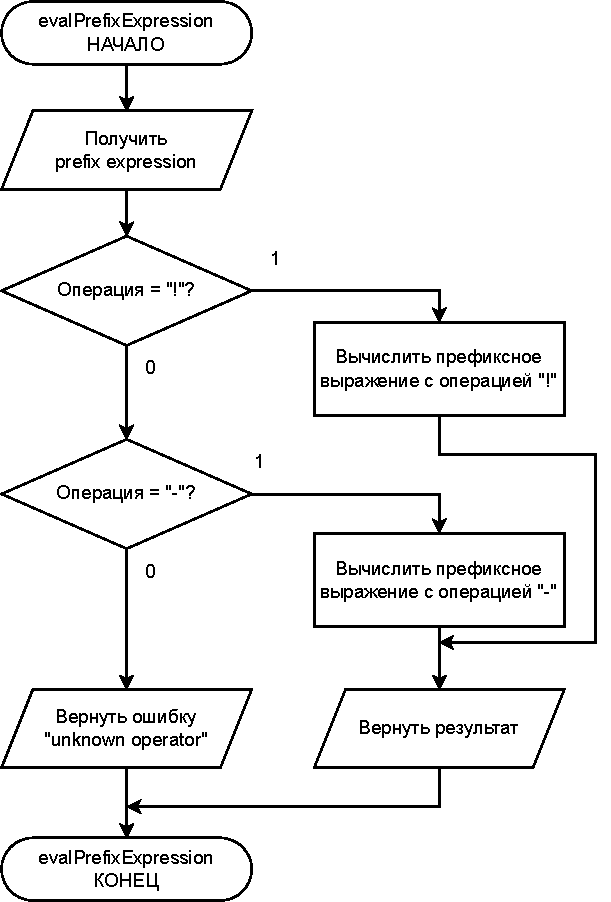
\includegraphics[width=0.9\textwidth]{structures/semantic_analyzer/semantic_prefix_expr.pdf}
	\caption{Схема алгоритма «evalPrefixExpression»}
	\label{f:semantic_prefix_expr}
\end{figure}

\clearpage

\begin{figure}[!htp]
	\centering
	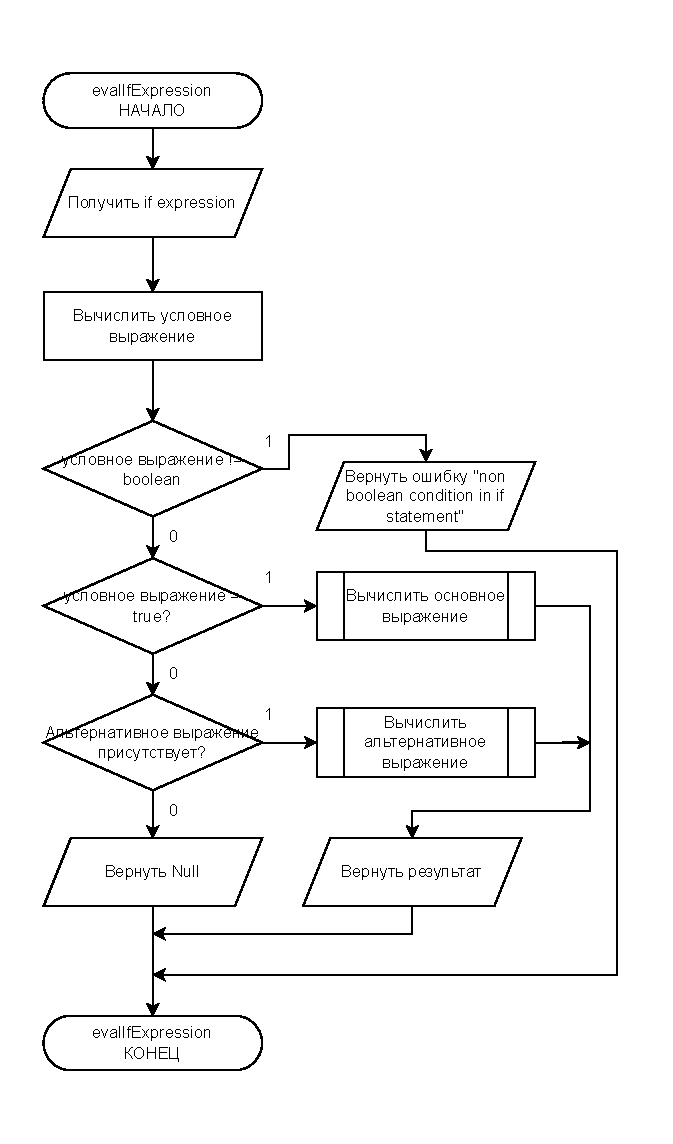
\includegraphics[width=0.7\textwidth]{structures/semantic_analyzer/semantic_if_expr.pdf}
	\caption{Схема алгоритма «evalIfExpression»}
	\label{f:semantic_if_expr}
\end{figure}

\clearpage

\begin{figure}[!htp]
	\centering
	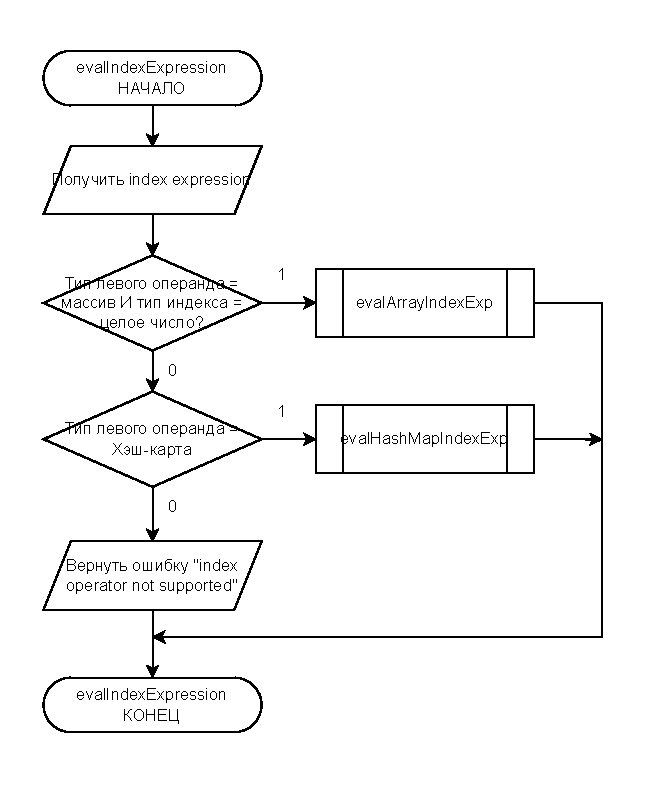
\includegraphics[width=0.75\textwidth]{structures/semantic_analyzer/semantic_index_expr.pdf}
	\caption{Схема алгоритма «evalIndexExpression»}
	\label{f:semantic_index_expr}
\end{figure}
\subsection{Разработка исполнителя}

Процесс вычисления выполняется над выражениями из узлов абстрактного синтаксического дерева.
Такой вид интерпретатора, который работает с AST называется <<tree walking interpreter>> или древовидный интерпретатор.
В таком интерпретаторе выполняется обход AST и выполнение соответствующих операций для каждого узла.

Последним этапом в процессе обработки исходного кода является его исполнение.
До этого шага все выражения языка представляют собой набор символов, токенов или ветви абстрактного синтаксического дерева без какого-либо семантического значения.
На данном этапе выражения языка приобретают смысл, то есть начинают интерпретироваться и действовать в соответствии с правилами и инструкциями языка.

Этап исполнения выполняется непосредственно после семантического анализа.
Если во время семантического анализа в обрабатываемом выражении не было обнаружено ошибок, выполняется переход к его вычислению.
Вычисление выражения выполняется в зависимости от его типа, например,
для инфиксного выражения применяется указанная в нем операция над левым и правым операндами и формируется результат в виде объекта соответствующего типа,
содержащего результат операции, а для условного выражения сначала вычисляется значение условия,
а затем в зависимости от его результата выполняется либо основная ветвь (при значении условия «true»), либо альтернативная (при значении условия «false»).

Только лишь вычислять значения выражений недостаточно.
Нужно также сохранять значения переменных для того, чтоб к ним можно было обратиться при обнаружении в выражениях.
Чтобы обеспечить эту возможность введем окружение – структуру данных, хранящую информацию о переменных и связанных с ними значениях на время выполнения программы.
Таким образом, при объявлении переменной, информация о ней будет записываться в окружение, а при необходимости получить значение этой переменой – ее значение будет считано из окружения.

В качестве примера работы алгоритма на рисунках~\ref{f:eval_int_infix_expr}~-~\ref{f:eval_string_infix_expr} приведены схемы алгоритма вычисления некоторых выражений.

\clearpage

\begin{figure}[!htp]
	\centering
	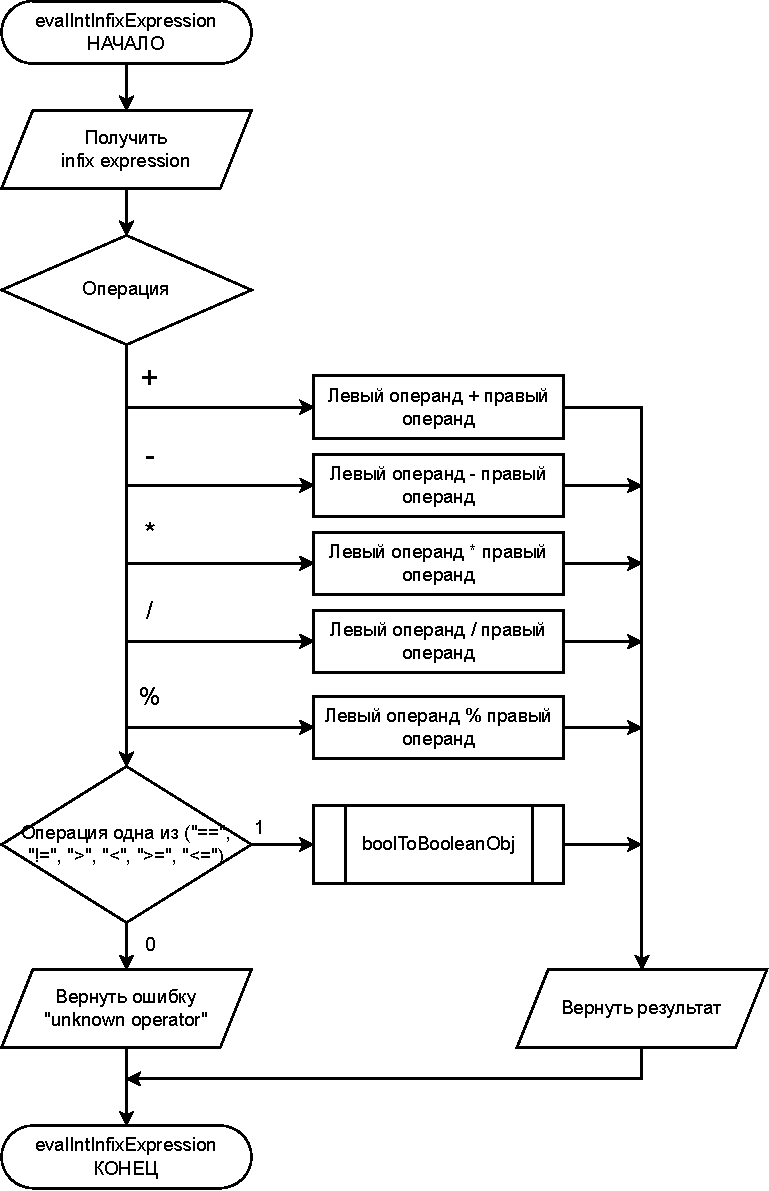
\includegraphics[width=0.8\textwidth]{structures/evaluator/eval_int_infix_expr.pdf}
	\caption{Схема алгоритма вычисления целочисленного инфиксного выражения}
	\label{f:eval_int_infix_expr}
\end{figure}

\clearpage

\begin{figure}[!htp]
	\centering
	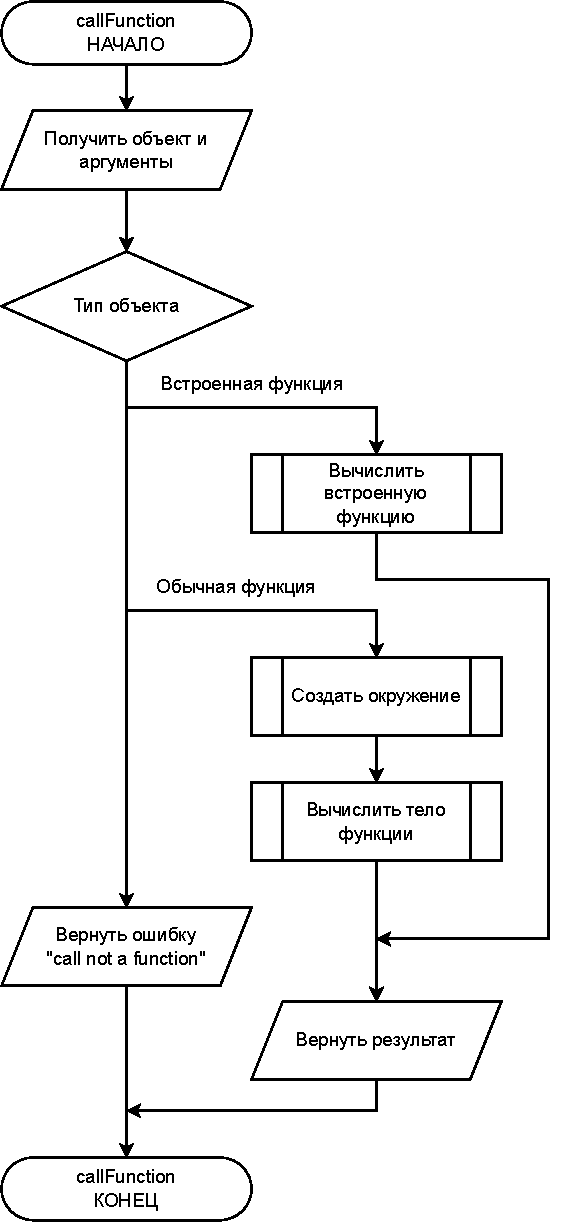
\includegraphics[width=0.6\textwidth]{structures/evaluator/eval_callFunction.pdf}
	\caption{Схема алгоритма исполнения вызова функции}
	\label{f:eval_callFunction}
\end{figure}

\clearpage

\begin{figure}[!htp]
	\centering
	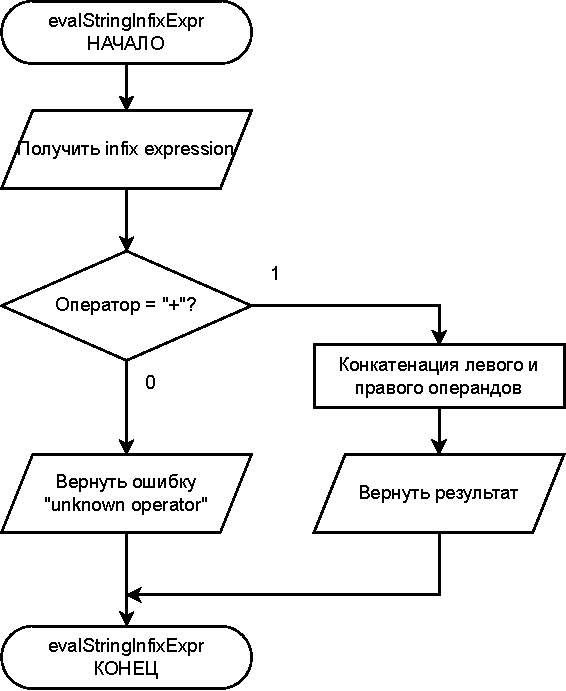
\includegraphics[width=0.5\textwidth]{structures/evaluator/eval_string_infix_expr.pdf}
	\caption{Схема алгоритма вычисления инфиксного выражения для строк}
	\label{f:eval_string_infix_expr}
\end{figure}

\section*{Вывод}

В данном разделе на основании разработанных архитектурно-структурных решениях и алгоритмах функционирования выполнена программная реализация модуля интерпретации предметно-ориентированного языка.
С помощью выбранных инструментов разработки выполнена программная реализация лексического анализатора, синтаксического анализатора, семантического анализатора и исполнителя.